\documentclass[twocolumn,8pt]{article}

\usepackage{amsmath}
\usepackage{enumerate}
\usepackage{array}
\usepackage[cm]{fullpage}
\usepackage{subfig}
\usepackage{graphicx}
\usepackage{float}
\usepackage{amsfonts}
\usepackage{setspace}
\usepackage{hyphenat}
\usepackage{multicol}
\usepackage{titlesec}
\usepackage{lettrine}
\usepackage[font={scriptsize,bf,sf}]{caption}
\usepackage{boxedminipage}
\usepackage{authblk}
\makeatletter
\renewcommand\AB@affilsepx{, \protect\Affilfont}
\makeatother

\addtolength{\oddsidemargin}{0.1in}
\addtolength{\evensidemargin}{0.1in}
\addtolength{\textwidth}{-0.3in}
%\setlength{\parskip}{1ex plus0.5ex minus0.2ex}
\setlength\parindent{10pt}
\setlength{\columnsep}{0.5cm}
\pagenumbering{gobble}

\titleformat{\section}
  {\normalfont\sffamily\normalsize\bfseries}{\thesection}{0.5em}{}

\titleformat{\subsection}[runin]
  {\sffamily\small\bfseries}{\thesubsection}{0.3em}{\addperiod}

\newenvironment{Figure}
  {\par\medskip\noindent\minipage{\linewidth}}
  {\endminipage\par\medskip}

\newcommand{\addperiod}[1]{#1.}

\title{\vspace{-1cm} \huge \sffamily \bfseries Social fluidity mobilizes contagion in human and animal populations}
\author[1]{\small \sffamily \bfseries Ewan Colman\thanks{\scriptsize \sffamily ec975@georgetown.edu}}
\author[2]{\small \sffamily \bfseries Vittoria Colizza}
\author[3]{\small \sffamily \bfseries Ephraim M. Hanks}
\author[4]{\small \sffamily \bfseries Andreas P. Modlmeier}
\author[4]{\small \sffamily \bfseries David P. Hughes}
\author[1]{\small \sffamily \bfseries Shweta Bansal}
\affil[1]{\footnotesize \sffamily Department of Biology, Georgetown University}
\affil[2]{\footnotesize \sffamily INSERM, Paris}
\affil[3]{\footnotesize \sffamily Department of Statistics, Pennsylvania State University}
\affil[4]{\footnotesize \sffamily Department of Entomology, Pennsylvania State University}

\date{\vspace{-5ex}}

\begin{document}
\openup -1em

\maketitle
\footnotesize
%\begin{multicols}{2}
\noindent
\textbf{\sffamily \fontdimen2\font=0.6ex Humans and other group-living animals tend to distribute their social effort heterogeneously; individuals predominantly interact with their closest companions while maintaining weaker social bonds with less familiar group members. By incorporating this heterogeneity into a mathematical model we find that a single parameter, which we refer to as \emph{social fluidity}, controls the level of social mixing in the population. Large values of social fluidity correspond to gregarious behavior whereas small values signify the existence of persistent bonds between individuals. To investigate how social behavior influences the likelihood of an epidemic outbreak we derive an analytical expression of the relationship between social fluidity and the basic reproductive number of an infectious disease. We compare social behavior across 12 species by applying the model to empirical human and animal social interaction data. For species that form strong social bonds, the model describes frequency-dependent transmission that is highly sensitive to changes in social fluidity. As social fluidity increases, animal-disease systems become increasingly density-dependent. Finally, based on a computational disease spread model on empirical social data, we find that social fluidity is a stronger predictor of disease outcomes than  both group size and connectivity.}
\vspace{0.5cm}
\small
\lettrine{S}ocial behavior is fundamental to the survival of many species such as ants, humans, and dolphins. It allows the formation of social groups providing fitness advantages from greater access to resources and better protection from predators \cite{krause2002living}. Within these groups structure emerges from the interactions that occur when individuals communicate across space, cooperate in sexual or parental behavior, or clash in territorial or mating conflicts \cite{10.2307/2800384}. While many animal societies have been studied independently \cite{sah106633}, some questions about the nature of social living can only be answered by comparing social behavior across a range of species \cite{dunbar2010bondedness}. This motivates the question: how can we compare the social behavior of one species to that of another?

Social animals typically have limited time and resources to invest in their relationships \cite{SUEUR2011156}. To compensate, the social effort of an individual tends to be distributed heterogeneously among the members of their group. Despite the growing evidence for this in human communication \cite{MacCarron2016151,saramaki2014persistence,10.1371/journal.pone.0022656}, attempts to quantify this aspect of sociality in animal systems are often challenged by unavoidable sampling biases \cite{10.2307/4535790}. Furthermore, while heterogeneous interaction frequencies and temporal dynamics such as circadian rhythms and bursty activity patterns have become common in social network models \cite{Holme2015}, realistic assumptions about how individuals distribute their social effort are rarely incorporated. 

\begin{figure}[b!]
\noindent
\begin{boxedminipage}{0.49\textwidth}
{\sffamily\large\bfseries Significance }\\

{\normalsize \sffamily The study of relationships within animal groups has provided many insights into the nature of social behavior. Despite this, finding a reliable measure of sociality that can be used to compare animal social systems has remained a challenge. We introduce \emph{social fluidity}, a measure of heterogeneity in how individuals choose to distribute their social effort across the group. We demonstrate the use of this measure by applying it to 57 social networks from 12 animal species. Our results indicate that social fluidity is a better predictor of disease spread than measures typically used in social network analysis such as the mean number of social ties or the size of a social group.}
\end{boxedminipage}
\end{figure}

When social interaction requires shared physical space it can also be a conduit for the transmission of infectious disease \cite{altizer2003social}. It is generally thought that if transmission occurs through the environment then the risk of epidemic is driven by group size (density-dependence) \cite{de1995does}, whereas if transmission requires close proximity encounters that only occur between bonded individuals then we expect social connectivity to determine the outcome (frequency-dependence) \cite{doi:10.1093/biosci/biw175}. In reality, however, animal-disease systems are not so easy to categorize \cite{patterson2013parasite}. For example, social ties must be created to maintain cohesiveness in a growing social group \cite{LEHMANN20071617}, implying that transmission through direct contact may in fact depend on population density. On the other hand, as social effort is distributed heterogeneously, low levels of social mixing may constrain the spread of the disease \cite{karsai2014time}.

Here, we introduce a mathematical model based on the concept of \emph{social fluidity} which we define as heterogeneity in the distribution of social effort. Using empirical data from previous studies, we estimate the social fluidity of a number of human and animal social systems. Using analytical and computational models of disease spread we show that social fluidity predicts disease outcomes better than other social behavioral indicators and spans the distance between density-dependent and frequency-dependent disease systems. 

\begin{figure*}
  \begin{minipage}[c]{0.67\textwidth}
    \includegraphics[width=\textwidth]{Figures/concept_fig.png}
  \end{minipage}\hfill
  \begin{minipage}[c]{0.3\textwidth}
  \caption{\textbf{Left:} Each individual can be represented as a single point on this plot. Dashed lines mark the boundary of the region where data points can feasibly be found. \eqref{degree} is plotted for two values of $\phi$ representing two possible types of social behavior; as the number of observed interactions grows, the set of social contacts increases; the rate at which it increases influences how we categorize their social behavior. \textbf{Middle:} The weight of the edges between $i$ and the other nodes represents the propensity of $i$ to interact with each of the other individuals in the population. \textbf{Right:} Probability distributions that correspond to the different levels of heterogeneity in the contact propensities, both distributions are expressed by \eqref{distribution}.}\label{concept_fig}
  \end{minipage}
\end{figure*}

\section*{Modeling social heterogeneity \& disease transmission}
Our objective is to measure social heterogeneity in a range of human and animal populations and provide an understanding of how social behavior influences the susceptibility of the group to infectious disease. We start by introducing a model that captures hidden elements of social dynamics (in particular, how individual group members distribute their social effort) and mathematically describe the relationships between social variables that are routinely found in studies of animal behavior (in particular, the number of social ties and the number of interactions observed). We then couple this social behavior model with a general model of infectious disease spread to expound the link between social behavior and disease outcomes.

\subsection*{Social behavior model}
\label{social_behavior}
Consider a closed system of $N$ individuals and a set of interactions between pairs of individuals that were recorded during some observation period. These observations can be represented as a network: an individual, $i$, is a \emph{node}; if at least one interaction between nodes $i$ and $j$ has been observed then we say that an \emph{edge} exists between them; the \emph{edge weight}, $w_{i,j}$, denotes the number of times this interaction was observed. The total number of times $i$ was observed interacting is denoted by \emph{strength}, $s_{i}=\sum_{j}w_{i,j}$, and the number of nodes with whom $i$ is observed interacting is its \emph{degree}, $k_{i}$.

We focus on one individual in the system, which we name the \emph{focal} node, $i$, and consider the $s_{i}$ interactions in which it participated. We define $x_{j|i}$ to be the probability that an interaction involving $i$ will also involve node $j$. Therefore the probability that at least one of these interactions is with $j$ is $1-(1-x_{j|i})^{s_{i}}$.

The main assumption of the model is that the values of $x_{j|i}$ over all $i,j$ pairs are distributed heterogeneously according to a probability distribution, $\rho(x)$\footnote{\scriptsize \sffamily $x_{j|i}$ are subject to network interdependencies. Specifically, $AX=X^{T}A$ and $X\textbf{1}=\textbf{0}$, where $X$ is a matrix whose $i,j$ entry is $-1$ if $i=j$ and $x_{j|i}$ otherwise, $A$ is any diagonal matrix with positive entries, and $\textbf{0}$ and $\textbf{1}$ are column vectors of length $N$ containing only $0$ and $1$, respectively. Thus, $\rho(x)$ is the distribution of marginal $x_{j|i}$ values of the joint distribution $P(X)$.}. Thus, after $s$ observed interactions of the focal node, the probability that an edge exists between the focal node and any other individual in the population is  
\begin{equation}
\label{i_to_any}
\Psi(s)=1-\int\rho(x)(1-x)^{s}dx.
\end{equation}
Our goal is to find a form of $\rho$ that accurately reproduces network structure observed in real social systems. Motivated by our exploration of empirical interaction patterns from a variety of species (Figure S1), we propose that $\rho$ has a power-law form:
\begin{equation}
\label{distribution}
\rho(x)=\frac{\phi\epsilon^{\phi}}{1-\epsilon^{\phi}}x^{-(1+\phi)} \text{ for } \epsilon<x<1,
\end{equation}
where $\phi$ ($>0$) controls the heterogeneity in the values of $x$, and $\epsilon$ simply truncates the distribution to avoid an asymptote at $x=0$. Combining \eqref{i_to_any} and \eqref{distribution} we find that
\begin{equation}
\label{hyper_solution}
\Psi(s,\phi,\epsilon)=1-\frac{\phi\epsilon^{\phi}(1-\epsilon)^{s+1}}{(1-\epsilon^{\phi})(s+1)}{}_{2}F_{1}(s+1, 1+\phi, s+2, 1-\epsilon)
\end{equation}
where the notation ${}_{2}F_{1}$ refers to the Gauss hypergeometric function \cite{absteg}. The value of $\epsilon$ is determined by $\sum_{j}x_{j|i}=1$ and therefore depends on $N$ and $\phi$ (\emph{Materials and Methods} \ref{lower_bound}). It follows that the degree of the focal node is determined by its activity rate, the level of heterogeneity in partner choice, and the size of the population (\emph{Materials and Methods} \ref{degree_dist}). More explicitly,
\begin{equation}
\label{degree}
\langle k \rangle=(N-1)\Psi(s,\phi,N)
\end{equation}
where $\langle k \rangle$ is the expected degree of the focal node.

The parameter $\phi$ controls the heterogeneity in  interaction frequencies and is therefore the main determinant of social mixing in the model. We use the term \emph{social fluidity} to refer to this quantity. Figure \ref{concept_fig} illustrates how the value of $\phi$ can create different types of social behavior. Low social fluidity ($\phi\ll 1$) would produce what we might describe as ``allegiant'' behavior: interactions with the same partner are frequently repeated at the expense of interactions with unfamiliar individuals. As $\phi$ increases, the model produces more ``gregarious'' behavior: interactions are repeated less frequently and the number of partners is larger. While this phenomena could be described as  ``social strategy'' or ``loyalty'' \cite{10.1371/journal.pcbi.1004152,miritello2013limited}, we feel that ``social fluidity'' is most appropriate for this work as it conveys an intuitive notion relevant to disease propagation \cite{Reluga20141901}.

\subsection*{Disease transmission model}
\label{disease_section}
Building on the social behavior model introduced in the previous section, we consider a model of disease transmission. We focus on the basic reproductive number $R_{0}$, defined as the mean number of secondary infections caused by a single infectious individual in an otherwise susceptible population. We first derive a formula for the individual reproductive number, $r(s_{i})$, in terms of the relative rate of activity of the individual, and define $R_{0}$ to be the mean of $\{r(s_{i})\}$ over the population. By calibrating the disease parameters in a way that controls for varying time-scales of activity in different populations, we obtain a result that quantifies the relative significance of social fluidity across a range of social systems including those driven by group size (density-dependent transmission) and those driven by group connectivity (frequency-dependent transmission).  

In our model, disease transmission requires an infected individual, $i$, who is social (i.e. has $s_{i}$ interactions during an observation period of duration $\Delta t$) and may interact with any other individual, $j$ (with probability $x_{j|i}$). When such an interaction occurs, $i$ will infect $j$ with probability $\beta$. The infectiousness of $i$ continues for a period of duration $\tau$, where $\tau$ is an exponentially distributed random variable with mean $1/\gamma$ (i.e. $\gamma$ is the recovery rate).

Assuming the interactions of $i$ are distributed randomly across the observation period, it follows that transmission events follow a Poisson process with rate $s_{i}x_{j|i}\beta/\Delta t$. Thus the probability that infection transmits from $i$ to any given $j$ is
\begin{equation}
\label{first_T}
T_{i\rightarrow j}(\tau,s_{i},x_{j|i})=1-\exp(s_{i}x_{j|i}\beta\tau/\Delta t).
\end{equation}
The reproductive number for $i$, $r(s_{i})$, is found by integrating \eqref{first_T} over all possible values of $\tau$ and $x_{j|i}$ then multiplying by the number of susceptible individuals, $N-1$ (SI Text). 

Instead of choosing infection parameter values that pertain to a specific disease or social system, we select values for each system separately in a way that exposes the effects of population size and social fluidity. We achieve this by setting the mean infectious period in such a way that would cause $R_{0}$ to be equal to the constant $R^{*}$ if the population was large and homogeneously mixed, i.e every interaction is with a new partner (\emph{Materials and Methods} \ref{disease_calib}). Consequently, social systems with a high interaction frequency are coupled with diseases that have relatively short mean infectious periods. 

After calibrating the parameters we can derive the following result for the reproductive number of an individual that was observed interacting $s$ times,
\begin{align}
\label{R_0_solution}
%\begin{split}
r(s)=&\frac{1-\phi}{\phi(\epsilon^{\phi}-\epsilon)}\left[1-\epsilon^{\phi}+\epsilon^{\phi}{}_{2}F_{1}(-\phi,1,1-\phi;-R^{*}s/\langle s \rangle)\right.\nonumber\\
&\left.-{}_{2}F_{1}(-\phi,1,1-\phi;-\epsilon R^{*}s/\langle s \rangle)\right],
%\end{split}
\end{align}
where $\langle s \rangle$ is the mean of $\{s_{i}\}$ over the population. In all the analysis presented we arbitrarily choose $R^{*}=2$. 

To further expose the dependencies between population density, social fluidity, and disease transmission we evaluate $N$ and $R_{0}$ over a range of $\epsilon$ and $\phi$ values (the formula for $N(\epsilon,\phi)$ is given in \emph{Materials and Methods} \ref{lower_bound} while for $R_{0}$ we assume $s=\langle s \rangle$ in \eqref{R_0_solution}). At small population sizes, $R_{0}$ increases with $N$ and converges as $N$ goes to $\infty$ (Figure \ref{disease_theory}\textbf{A}). The rate of this convergence increases with $\phi$. When $\phi<1$, the limit of $R_{0}$ is a function of $\phi$ (Figure \ref{disease_theory}\textbf{B}). At these values of $\phi$, the individual will choose to repeat interactions despite having the choice of infinitely many potential interaction partners. When $\phi>1$ and the population is large the probability of a repeated interaction falls to zero and we have that $R_{0}=R^{*}$.

\begin{figure}[h!]
\centering
\includegraphics[width=\linewidth]{Figures/disease_theory.png}
\captionof{figure}{\textbf{A:} Theoretical results from \eqref{R_0_solution}; the relationship between $R_{0}$ and population size is shown to depend on the value of $\phi$. Dashed lines show the limit for large $N$.  \textbf{B:} In large populations $R_{0}$ increases with $\phi$ up to $\phi=1$. Beyond this value, infections occur as frequently as they would in a homogeneously mixed population.}
\label{disease_theory}
\end{figure}
%\section*{Data-driven insights on social heterogeneity \& disease potential}
\section*{Social behavior \& disease spread in empirical systems}
The previous section introduced a model of social behavior in which social fluidity, $\phi$, quantifies heterogeneity in the way individuals distribute their social effort among other members of the population. To understand the results of the model in the context of real systems we estimate $\phi$ in $57$ networks from $19$ studies of human and animal social behavior (\emph{Materials and Methods}) \cite{isella2011s,
10.1371/journal.pone.0023176,
10.1371/journal.pone.0136497,
10.1371/journal.pone.0073970,
10.1371/journal.pone.0020298,
Carter20122573,
Davis20141004,
%borremans2016nonlinear,
Grant1973449,
levin2016stress,
sailer1984proximity,
mourier2017learning,
massen2013stability,
sade1972sociometrics,
butovskaya1994structure,
takahata1991diachronic,
hass1991social,
lott1979dominance,
SCHEIN195545,
hobson2015social}. 

We focus our attention to those interactions which are capable of disease transmission (i.e. those that, at the least, require close spatial proximity). Each dataset provides the number of interactions that were observed between pairs of individuals (SI Text). We assume that the group size, $N$, is equal to the number of individuals observed in at least one interaction. Figure S1 shows the data and the distribution fitted using maximum likelihood estimation. 

The model provides a good fit to every dataset; the worst fitting animal social network agrees with the model better than synthetic data generated $92\%$ from model simulation and $8\%$ from random noise (SI Text). For comparison, the model was also applied to $9$ networks generated from social media data \cite{Charlton160162}, $3$ of which showed less agreement with the model than any of the non-electronic networks (SI Text). Since agreement between the model and the data is therefore not a certainty, it is remarkable that the social fluidity model is applicable to such a wide range of animal social networks.

\begin{figure}[t]
\centering
\includegraphics[width=\linewidth]{Figures/interaction_types.png}
\captionof{figure}{Each point represents a human or animal system for which social fluidity was estimated. Results are organized by interaction type: aggression includes fighting and displays of dominance, food sharing refers to mouth-to-mouth passing of food, antennation is when the antenna of one insect touches any part of another, space sharing interactions occur with spatial proximity during foraging, face-to-face refers to close proximity interactions that require individuals to be facing each other, association is defined as co-membership of the same social group.}
\label{phi_for_all_networks}
\end{figure}

\begin{figure*}[t]
	\centering
	\includegraphics[width=0.9\textwidth]{Figures/R0_for_all_networks.png}\qquad
  	\caption{Each point represents a human or animal data-set for which the time of interactions appear in the data. For each individual, $i$, in a population, the mean number of secondary infections is obtained from simulation and the mean, $R_{0}$ ($\pm$ one standard error in part \textbf{A}), is plotted against metrics of social structure. Note that the parameters in the disease simulation have been calibrated with the rate of activity of each system to make these metrics comparable.}
.\label{disease_simulation_fig}
\end{figure*}

\subsection*{Characterizing social fluidity}
Figure \ref{phi_for_all_networks} shows the estimated values of $\phi$ for all our study populations. We organize the measurements of social fluidity by interaction type. Aggressive interactions have the highest fluidity (which implies that most interactions are rarely repeated with the same individuals), while grooming interactions have the lowest (which implies frequent repeated interactions with the same individuals). Social fluidity also appears to be related to species: ant systems cluster around $\phi=1$, voles around $\phi=0.7$, humans around $\phi=0.6$ (with the exception of lower values observed in the high school data and the last day of a conference). However, we do not find that social fluidity is highly correlated with sociality type \cite{pratha_jae}. This is illustrated by the sizable difference in social fluidity between the sheep, bison, and cattle versus the kangaroos and bats all of which are categorized as fission-fusion species.

There is no significant correlation between the mean number of observations per individual, $\bar{s}$, and $\phi$ (Pearson $R^{2}=0.04$, $p=0.14$), which implies that sample size does not affect the estimate (Figure S2\textbf{A}). Larger populations tend to have smaller social fluidity values (Pearson $R^{2}=0.205$, $p<0.001$), however, this correlation is dependent on the presence of a few large populations in our data ($N>200$) (Figure S2\textbf{B}). Larger values of $\phi$ correspond to higher mean degrees (Pearson $R^{2}=0.16$, $p=0.002$) and less heterogeneity in the distribution of edge weights (measured as the variance divided by the mean $\sigma_{w}^{2}/\langle w\rangle$)  (Pearson $R^{2}=0.339$, $p=0.001$) (Figure S2\textbf{C} and \textbf{D}). Incidentally, weight heterogeneity and mean degree are uncorrelated in these data (Pearson $R^{2}=0.005$, $p=0.568$) implying that $\phi$ combines two distinct features of social behavior.

\subsection*{Impact of social fluidity on disease transmission}
To test the validity of the model and examine the utility of $\phi$ as an indicator of disease outcomes we simulated the spread of disease based on the interactions that occurred in the empirical data (\emph{Materials and Methods} \ref{simulation}). We assume that all individuals are equally likely to introduce the infection to the group. In doing so we avoid biasing our choice of infection seed to those who are more socially active (our results are therefore not influenced by degree heterogeneity). Thus, the basic reproductive number, $R_{0}$, is defined simply as the mean of the individual reproductive numbers over the entire population.

For each individual, $i$, we compared the simulated number of secondary infections to the prediction for $r(s_{i})$ given by \eqref{R_0_solution}. A small amount of error was observed (between $0.1$ and $0.258$ with one outlier at $0.344$) and the prediction consistently overestimated $R_{0}$ in human systems (Table S3), possibly because of the bursty nature of human contact \cite{karsai2011small}. Despite this, our overall conclusions from the disease simulation are consistent with the predicted results.

Figure \ref{disease_simulation_fig} shows that $\phi$ correlates with (simulated) $R_{0}$ better than other network metrics. Since $R^{*}$ ($=2$) represents the expectation of $R_{0}$ in a homogeneously mixed population of infinite size, the difference between $R_{0}$ and $R^{*}$ can be attributed to the effects of social fluidity and population size. Because the association between $\phi$ and $R_{0}$ is strong (shown in Figure \ref{disease_simulation_fig}\textbf{A}), the relationship between each of the other metrics and $R_{0}$ is qualitatively the same as the their relationship with $\phi$. Consequently, $R_{0}$ tends to be smaller in the largest populations (Figure \ref{disease_simulation_fig}\textbf{B}), suggesting that population size is not an important variable at such low values of $\phi$. For $\phi>1$, however, analytical results suggest that $N$ plays a larger role in determining $R_{0}$ (Figure S3).

The relative weakness of the correlation between mean degree and $R_{0}$ (Figure \ref{disease_simulation_fig}\textbf{C}) suggests that the interaction dynamics taking place \emph{on} each edge contribute significantly to the disease outcomes. For example, after transmission has occurred from one individual to another, repeats of the same interaction serve no advantage for the disease (most directly-transmitted infections are not dose-dependent). Since a large edge weight implies a high frequency of repeated interactions, networks with a higher mean weight tend to have lower values of $R_{0}$ (Figure \ref{disease_simulation_fig}\textbf{D}). Furthermore, heterogeneity in the distribution of weights concentrates a yet larger proportion of interactions onto a small number of edges, thus causing more repeat interactions and reducing $R_{0}$ (Figure \ref{disease_simulation_fig}\textbf{E}). 

\section*{Discussion}
We have defined a measure of fluidity in social behavior which quantifies how much mixing exists within the social relationships of a population. While social networks can be measured with a variety of metrics including size, connectivity, interaction heterogeneity and frequency, our methodology succeeds in reducing all such factors to a single quantity allowing comparisons across a range of human and animal social systems. Social fluidity correlates with both the density of social ties (mean degree) and the heterogeneity in the strength of those ties, yet they are not correlated with each other; this implies that social fluidity combines two distinct elements of social network analysis. We have also shown that this metric is a better predictor of $R_{0}$ than these other network metrics.

By measuring social fluidity across a range of human and animal systems we are able to rank social behaviors. In particular, we identify aggressive interactions as the most socially fluid; this indicates a possible learning effect whereby each aggressive encounter is followed by a period for which individuals avoid further aggression with each other \cite{parker1974assessment}. At the opposite end of the scale, we find interactions that strengthen bonds (and thus require repeated interactions) such as grooming in monkeys \cite{seyfarth1984grooming} and food-sharing in bats \cite{Carter20122573}. The fact that food-sharing ants are far more fluid than bats, despite performing the same kind of interaction, reflects their eusocial nature and the absence of any need to maintain long-lasting bonds with their kin \cite{holldobler2009superorganism}.

Most studies that aim to describe and quantify social structure are met with a number of challenges. The degree of an individual, for example, is known to scale with the length of the observation period \cite{perra2012activity}. By focusing not on the absolute value of degree, and instead focusing on how degree scales with the number of observations, our analysis controls for this bias. As with other network measures, however, social fluidity estimates lose reliability when only a sample of the group has been observed \cite{SILK20151}. Another hurdle in previous work has been the assumption that observed interactions will persist into the future \cite{perreault2010note}. Our method assumes only that the distribution of relationships remains constant through time, an assumption that is consistent with growing evidence \cite{miritello2013limited,10.1371/journal.pone.0173110}.

In trying to elucidate the connection between social behaviors and the spread of disease the first question to ask is whether the type of interactive behavior that the species participates in enables transmission of the infection. If it does, then the next important variable is the frequency of these interactions. Beyond this, other proposed influences include the number of social ties \cite{Craft20140107}, which we have shown to be less significant than social fluidity; modularity, which has previously been exposed as an unreliable predictor of disease outcomes \cite{sah2017unraveling}; and group size \cite{rifkin2012animals}, which we have shown to only be relevant in highly fluid populations. 

The relative significance of social fluidity becomes apparent when we compare the largest human face-to-face interaction system (\verb|highschool_0| in Tables S2 and S3 $N=312$, $R_{0}=0.99$, $\phi=0.422$), to the smallest (\verb|hospital_1|, $N=49$, $R_{0}=1.129$, $\phi=0.592$). Despite the former containing more than $6$ times as many individuals as the latter, its lower social fluidity causes $R_{0}$ to be a smaller. Similarly, the mean degree of the hospital data ($\bar{k}=5.1$) is more than double that of the first day of the conference (\verb|conference_0|, $\bar{k}=2.5$, $R_{0}=0.173$, $\phi=0.631$), yet the relatively small decrease in $\phi$ is enough to reduce the value of $R_{0}$. Thus, the risks associated with group size and the density of social ties are easily offset by minor changes in the way individuals choose to distribute their social effort. If the survival of a group depends on its size or its connectivity then this social adaptation can be made with little impact on the disease risks. 

Although social fluidity predicts the basic reproductive number $R_{0}$ better than alternative network-based metrics, this does not necessarily imply that it would be a good predictor of the final epidemic size in a population with higher-order social structure (e.g. clustering, degree heterogeneity) \cite{Millerrsif.2008.0524}. Even so, there are implications of this work that may improve the way epidemics are modeled. The growing evidence that human and animal interaction follows basic universal principals, such as constraints on the social capacity of an individual, ought to be encoded into infectious disease models that aim to achieve a coupling of social and disease dynamics \cite{bioglio2016recalibrating,masuda2017introduction}.

Unlike previous work that explores the disease consequences of population mixing \cite{Volz2925,Reluga20141901}, our analysis allows us to compare its effect across a range of social systems. We see, for example, the relationship between mixing and how disease risks scale with population size. For social systems that have high values of social fluidity, $R_{0}$ is highly sensitive to changes in $N$, whereas this sensitivity is not present at low values of $\phi$. Thus, both density dependent and frequency dependent disease dynamics are realized through the same model. Since many empirical studies support a transmission function that is somewhere between these two modeling paradigms \cite{Smith12052009,ECY:ECY20139492076,borremans2016nonlinear}, the modeling approaches applied in this study may be useful in informing transmission relationships in future disease studies.

\scriptsize
\section*{Materials and Methods}
Extended methods are provided in the SI Text
\renewcommand\thesubsection{\Alph{subsection}.}
\subsection{Computing the lower bound in \eqref{distribution}}
\label{lower_bound}
The value of $\epsilon$ is determined by the choice of $\phi$ and the value of $N$. Since interactions are pairwise, when $i$ interacts exactly one other individual is involved. Thus, the sum of the $x_{j|i}$'s over all other members of the population, $j$, is equal to $1$. We choose to express this as a constraint in expectation, with $(N-1)\langle x \rangle=1$,
where $\langle x \rangle$ denotes the mean of the distribution $\rho(x)$. This leads to 
\begin{equation}
\label{x_mean}
N=1+\frac{(1-\phi)(1-\epsilon^{\phi})}{\phi\epsilon^{\phi}(1-\epsilon^{1-\phi})}.
\end{equation}
We can therefore find $\epsilon$ for any give $N$ and $\phi$ by solving $(C+1)\epsilon^{\phi}-\epsilon-C=0$,
where $C=(1-\phi)/(N-1)\phi$, using the \emph{fsolve} function from the \emph{scipy.optimize} Python library (SI text). 

\subsection{Conditional degree distribution} 
\label{degree_dist}
The degree of $i$ is determined by $N-1$ independent Bernoulli trials, each with success probability $\Psi(s_{i})$. The probability that an individual will have degree $k$ given that they have interacted $s$ times, for any value of the global parameter $\phi$ is therefore given by
\begin{equation}
 P(k|s,\phi)=\binom{N-1}{k}\Psi(s,\phi)^{k}\left(1-\Psi(s,\phi)\right)^{N-1-k}.
\end{equation}
However, since this distribution gives non-zero probabilities for cases where $k>s$, which are invalid, we instead use
\begin{equation}
P(k|s,\phi)=\binom{s}{k}\left(\frac{(N-1)\Psi(s,\phi)}{s}\right)^{k}\left(1-\frac{(N-1)\Psi(s,\phi)}{s}\right)^{s-k}
\end{equation}
when if $0<s<N$. To evaluate the hypergeometric function in \eqref{hyper_solution} we used the \emph{hyp2f1} function  from the \emph{scipy.special} Python library.

\subsection{Parameter estimation}
\label{estimation}
%We use maximum likelihood estimation to fit the social behavior model to empirical data on interactions in a social group, and return the social fluidity $\phi$.
For each individual in a study population we know the number of times they interacted, $s_{i}$, and the number of partners with whom they interacted, $k_{i}$, in vector notation $\textbf{k}=\{k_{1},k_{2},...,k_{N}\}$ and $\textbf{s}=\{s_{1},s_{2},...,s_{N}\}$. The marginal log-likelihood function is
\begin{equation}
\log \mathcal{L}(\phi|\textbf{k},\textbf{s})=\sum_{i=1}^{N}\log[P(k_{i}|s_{i},\phi)].
\end{equation}
We then compute the maximum likely estimate $\phi=\text{argmax}_{\phi}\log \mathcal{L}(\phi|\textbf{k},\textbf{s})$. Our estimation is based on the marginal distribution of the degree of each node and does not take into account the interdependencies of the network structure. As such, we do not report standard errors or confidence intervals for our point estimates. For discussion of the use of marginal distributions in likelihood estimation see \cite{varin2011overview}.

The goodness-of-fit is calculated by comparing its likelihood to the likelihood of a null model in which the degree of each individual is a uniformly distributed random integer within the range of feasible values (SI Text).

\subsection{Disease model calibration}
\label{disease_calib}
We choose $\gamma$ for every system such that $R_{0}$ is equal to a fixed value, $R^{*}$, under the assumption of no effect from social fluidity and population size (i.e. in a large population with homogeneous mixing). Calibration is achieved when $\gamma$ is chosen to be  
\begin{equation}
\label{calibration}
\gamma=\frac{\beta\langle s\rangle}{ \Delta_{t} R^{*}}
\end{equation}
where $\Delta_{t}$ is the duration of the time-frame of the data and $\langle s\rangle$ is the mean of $s_{i}$ over the whole population. The effect of this calibration is that the recovery rate, $\gamma$, is proportional to the mean activity rate.

\subsection{Disease simulation}
\label{simulation}
Disease simulations were only performed on data for which the time of every interaction is recorded. Since the  transmission probability, $\beta$, and the rate of recovery, $\gamma$, are calibrated through \eqref{calibration}, the choice of $\beta$ does not affect $R_{0}$. We arbitrarily chose $\beta=1/4$. We report mean absolute error $|e|$, which is the mean difference between the analytical and simulated values of $r(s_{i})$, computed across $10^3$ simulations for each node. An extensive description is provided in the supplement (SI Text).

\subsection*{Acknowledgments} This work was supported by NSF grant number 1414296. We are grateful for insightful feedback from Pratha Sah. We also thank all the researchers who have made their behavioral data openly accessible, making this study possible.

%\end{multicols}

\qquad

%\begin{multicols}{2}
\sffamily
\tiny
% Bibliography
\bibliography{bibfile_5}
\bibliographystyle{unsrt}

%\end{multicols}
\end{document}
